\documentclass[10pt,letterpaper]{article}
\usepackage[margin=0.65in]{geometry}
\usepackage{graphicx}
\usepackage{booktabs}
\usepackage{amsmath}
\usepackage[hidelinks]{hyperref}
\usepackage{caption}
\captionsetup{font=normalsize,labelfont=bf}
\setlength{\parindent}{0pt}
\setlength{\parskip}{5pt}
\begin{document}

The L1 figure uses Experiment~1's whole-tensor canonical layouts, stratified over all
score components before profiling. The H100 L1 comparison uses the issue
quotient $Q_{32\mathrm{B}}$, matching the counter's 32-byte sector
unit.\footnote{NVIDIA Nsight Compute, \href{https://docs.nvidia.com/nsight-compute/ProfilingGuide/index.html}{Profiling Guide: metrics and memory workload analysis}.}
It gives perfect rank agreement for all six kernels with layout variation;
correlations with downstream L2 activity are less uniform.

\begin{figure}[!htbp]
\centering
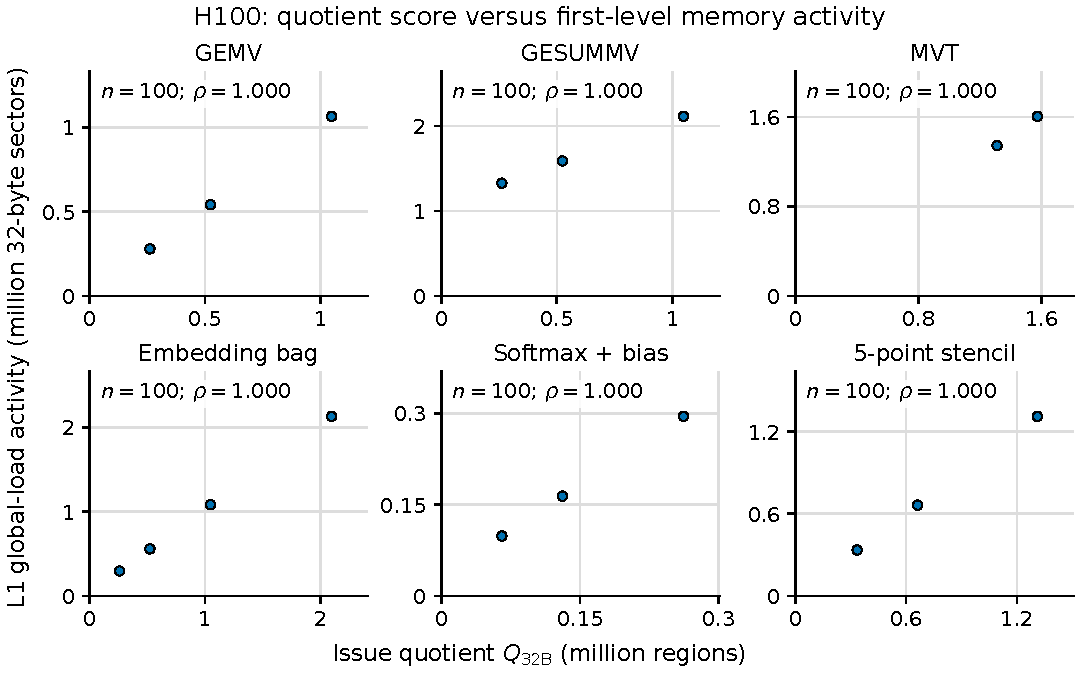
\includegraphics[width=\linewidth]{h100-quotient-l1.pdf}
\caption{Issue quotient versus first-level memory activity for all six pilot
kernels on NVIDIA H100. The horizontal axis is the target operand's dynamic
issue quotient $Q_{32\mathrm{B}}$ (component
\texttt{issue.g32.stream.load.32B}); the vertical axis is whole-kernel global-load
L1TEX sectors, measured by
\texttt{\detokenize{l1tex__t_sectors_pipe_lsu_mem_global_op_ld.sum}}.
Both axes use millions and start at zero; panel scales differ.
Each point is one distinct whole-tensor canonical mapping from the
all-scope-stratified Experiment~1 panel. Repeated coordinates overlap;
$n$ counts mappings, not visible markers. Points are medians of three
independent profiler-launch medians, each over 20 steady-state dispatches
under the warm-cache protocol. All three launch medians coincide for every mapping, so error bars
have zero height. Spearman's $\rho$ uses average ranks for ties.
The quotient scores only the varied operand, whereas the counter includes
all kernel loads; offsets therefore need not vanish.}
\label{fig:pilot-h100-l1}
\end{figure}

\clearpage
The L2 comparison summarizes the recorded pre-packet pilot results for
$G_C$ (Experiment~1) and $GL(p,2)$ (Experiment~3), using the median
correlation across six kernels.

\begin{table}[htbp]
\centering
\begin{tabular}{@{}lrr@{}}
\toprule
Kernel & H100 & MI300A \\
\midrule
GEMV & 0.299 & 0.977 \\
GESUMMV & 0.442 & 0.727 \\
MVT & 0.771 & 0.935 \\
Embedding bag & 0.966 & 0.988 \\
Softmax + bias & 0.959 & 1.000 \\
5-point stencil & 0.931 & 0.999 \\
\midrule
Median & 0.851 & 0.982 \\
\bottomrule
\end{tabular}

\caption{Median per-kernel Spearman correlations between $J_{\mathrm{area}}$
and L1-to-L2 read requests, using each device's \texttt{l1\_to\_l2} tau profile
and all-scope stratification. $G_C$ denotes Experiment~1's whole-tensor
canonical layouts; $GL(p,2)$ denotes Experiment~3's invertible binary
inner-tile layouts with row-major outer tiles.
Each cell is the median of six per-kernel correlations (bias+ReLU excluded),
each computed across 100 distinct mappings with average ranks for ties.
H100 uses \texttt{\detokenize{lts__t_requests_srcunit_tex_op_read.sum}};
MI300A uses \texttt{TCP\_TCC\_READ\_REQ\_sum}.
Each counter observation is the median of three independent profiler-launch
medians, each over 20 steady-state dispatches with warm caches.
These are recorded pre-packet pilot results; device-specific tau weights
were fitted using pilot counters.}
\label{tab:pilot-l2}
\end{table}

\end{document}
